\documentclass[11pt,a4paper]{article}

% ---------------------------------------------------------------------------
% The complexity of complete irreducible autocatalytic families:
% output-polynomial enumeration of irreducible RAFs if and only if P = NP.
%
% Author metadata: set the macros below before submission.
% \CompanionAuthor fills the author field of the companion-manuscript
% citations in refs.bib (certification2026, minraf2026).
% ---------------------------------------------------------------------------
\newcommand{\PaperAuthor}{Anonymous manuscript}
\newcommand{\PaperAffiliation}{}
\newcommand{\PaperDate}{14 September 2026}
\newcommand{\CompanionAuthor}{Anonymous manuscript}

\usepackage[T1]{fontenc}
\usepackage[utf8]{inputenc}
\usepackage{lmodern}
\usepackage{microtype}
\usepackage[a4paper,margin=1.05in]{geometry}
\usepackage{amsmath,amssymb,amsthm}
\usepackage{booktabs}
\usepackage{array}
\usepackage{enumitem}
\usepackage{xcolor}
\usepackage{tikz}
\usetikzlibrary{arrows.meta,positioning,calc,fit,backgrounds}
\renewcommand{\topfraction}{0.9}
\renewcommand{\textfraction}{0.05}
\renewcommand{\floatpagefraction}{0.75}
\usepackage[obeyspaces,spaces]{url}
\usepackage[numbers,sort&compress]{natbib}
\usepackage[colorlinks=true,linkcolor=blue!55!black,citecolor=blue!55!black,urlcolor=blue!55!black]{hyperref}
\hypersetup{pdftitle={The complexity of complete irreducible autocatalytic families: output-polynomial enumeration of irreducible RAFs if and only if P = NP},
 pdfauthor={\PaperAuthor},
 pdfsubject={Enumeration complexity of irreducible RAFs in catalytic reaction systems},
 pdfkeywords={autocatalytic sets, RAF theory, enumeration complexity, output-polynomial time, satisfiability, formal verification}}

\providecommand{\doi}[1]{}
\renewcommand{\doi}[1]{\href{https://doi.org/#1}{\nolinkurl{doi:#1}}}

\setlist{itemsep=2pt,topsep=3pt}
\setlength{\emergencystretch}{1.5em}

\theoremstyle{plain}
\newtheorem{theorem}{Theorem}[section]
\newtheorem{proposition}[theorem]{Proposition}
\newtheorem{lemma}[theorem]{Lemma}
\newtheorem{corollary}[theorem]{Corollary}
\theoremstyle{definition}
\newtheorem{definition}[theorem]{Definition}
\newtheorem{construction}[theorem]{Construction}
\newtheorem{example}[theorem]{Example}
\theoremstyle{remark}
\newtheorem{remark}[theorem]{Remark}
\newtheorem{question}[theorem]{Question}

\DeclareUrlCommand\lean{\urlstyle{tt}}

\newcommand{\Irr}{\mathcal I}
\newcommand{\cl}{\operatorname{cl}}
\newcommand{\RAF}{\operatorname{RAF}}
\newcommand{\maxRAF}{\operatorname{maxRAF}}
\newcommand{\Avail}{\operatorname{Avail}}
\newcommand{\PP}{\mathsf P}
\newcommand{\NP}{\mathsf{NP}}
\newcommand{\coNP}{\mathsf{coNP}}
\newcommand{\sharpP}{\#\mathsf P}
\newcommand{\bits}{\operatorname{bits}}
\newcommand{\mask}{\operatorname{mask}}
\newcommand{\SAT}{\textup{\textsc{Sat}}}
\newcommand{\Exact}{\textup{\textsc{Exact}}}
\newcommand{\Extra}{\textup{\textsc{Extra}}}
\newcommand{\cG}{\mathcal G}
\newcommand{\cA}{\mathcal A}
\newcommand{\Nat}{\mathbb N}
\newcommand{\true}{\mathbf 1}

\title{The complexity of complete irreducible autocatalytic families:\\
output-polynomial enumeration of irreducible RAFs\\ if and only if $\PP=\NP$}
\author{\PaperAuthor\\ \PaperAffiliation}
\date{\PaperDate}

\begin{document}
\maketitle

\begin{abstract}
An irreducible reflexively autocatalytic and food-generated set (irreducible RAF, or irrRAF) is an inclusion-minimal nonempty RAF of a finite catalytic reaction system. Detecting whether a system contains a RAF is polynomial, and Steel, Hordijk and Smith (\emph{J.\ Theor.\ Biol.}, 2013) gave a deletion-based criterion for certifying that a supplied list of irreducible RAFs is complete, whose cost grows exponentially in the list length. We settle the complexity of listing the complete family. For finite catalytic reaction systems with an explicit incidence encoding, a fixed deterministic multitape Turing machine that writes every irreducible RAF exactly once in time polynomial in the input length plus the output length exists if and only if $\PP=\NP$. The lower bound is a polynomial-size SAT source whose \emph{entire} RAF family has a prescribed normal form: a mandatory catalytic cycle forces all auxiliary reactions into every RAF, and a reset reaction cannot enable itself, so the irreducible RAFs are exactly $n$ conflict pairs together with the satisfying assignments of the formula. Unsatisfiable formulas therefore have a known polynomial-size complete family, and an output-sensitive time bound becomes a polynomial deadline that decides satisfiability. The converse builds, under $\PP=\NP$, a uniform enumerator from a polynomial-size supported-trace SAT encoding of the query ``is there a RAF avoiding every known output?'' and a filtered deletion minimizer. The same source gives an exact count identity $|\Irr(Q_\varphi)|=n+\#\SAT(\varphi)$, coNP-completeness of exact certification, $\sharpP$-hardness of counting, and an equivalence between polynomial-delay streaming enumeration and $\PP=\NP$. The classification is machine-checked in Lean~4 for concrete multitape machines, including original-input initialization, arbitrary finite identifiers, and a count-prefixed fixed-width output, with no hypotheses beyond the standard axioms.
\end{abstract}

\noindent\textbf{Keywords.} autocatalytic sets; RAF theory; catalytic reaction systems; enumeration complexity; output-polynomial time; irreducible RAFs; satisfiability; formal verification.

\medskip
\noindent\textbf{MSC 2020.} 68Q17, 68Q25, 92E20, 05C65, 68V20.

\section{Introduction}\label{sec:intro}

Reflexively autocatalytic and food-generated sets (RAFs) are a finite combinatorial model of collectively self-sustaining reaction networks. The concept goes back to Kauffman's autocatalytic sets of proteins \cite{kauffman1986autocatalytic,kauffman1993origins}, was given its present form by Hordijk and Steel \cite{hordijk2004detecting}, and has since developed into a structural theory with efficient algorithms \cite{hordijk2012structure,hordijk2015algorithms,steel2019autocatalytic,steel2020structure,steel2023interior} and applications to early metabolism and the origin of life \cite{hordijk2017chasing,hordijk2018life,xavier2020autocatalytic,sousa2015ecoli}. A catalytic reaction system consists of molecule types, reactions with reactants and products, a food set of freely available molecules, and a catalysis relation. A nonempty set of reactions is a RAF if all of its reactants can be built up from the food by reactions of the set, and each of its reactions is catalysed by a molecule that is food or is produced by the set.

Because unions of RAFs are RAFs, a system that contains a RAF contains a unique largest one, the \emph{maxRAF}, and the RAF algorithm of Hordijk and Steel computes it in polynomial time \cite{hordijk2004detecting}. The \emph{minimal} autocatalytic subsystems point in the opposite direction. Steel, Hordijk and Smith \cite{steel2013minimal} studied the irreducible RAFs (irrRAFs), which contain no proper RAF, and the smallest RAF overall. They proved that finding a RAF of minimum size is NP-hard, showed that a single irreducible RAF can be found in polynomial time by a deletion sweep, and gave a criterion for certifying that a supplied list of $k$ irreducible RAFs is complete: the list is complete if and only if deleting one reaction from each listed set, in every possible way, always leaves a system with no RAF. That test needs up to $\prod_i|I_i|$ maxRAF computations, and they asked whether this dependence on $k$ can be improved \cite[Section~6.1]{steel2013minimal}. Hordijk's recent preprint develops exhaustive and randomized methods for enumerating irreducible and closed autocatalytic sets \cite{hordijk2026enumerating}. The complete irreducible family is the natural object behind all of these questions: by an elementary argument (Proposition~\ref{prop:survival}) it determines exactly which reaction deletions leave a RAF, and its members are the minimal structural cores that any downstream chemical or biological analysis begins from.

Finding one irreducible RAF and listing the complete family are different computational tasks. A complete family can be exponentially large, but that observation alone does not rule out an algorithm whose running time is polynomial in the input \emph{and the output it must write}; this is the usual output-polynomial (or \emph{output-sensitive}) standard for enumeration problems \cite{johnson1988generating,strozecki2023enumeration}. The question this paper answers is whether such a guarantee can hold uniformly over all finite catalytic reaction systems.

\subsection{Main result}

Throughout, $Q=(M,R,F,\rho,\pi,C)$ is a finite catalytic reaction system with molecule set $M$, reaction identifier set $R$, food set $F\subseteq M$, reactant and product maps $\rho,\pi\colon R\to 2^M$, and catalysis relation $C\subseteq M\times R$. We write $\Irr(Q)$ for the family of its irreducible RAFs, and we fix the explicit encoding of Definition~\ref{def:encoding}: the input is a dense bit string of length $N=2d+r+2+3dr$ for $d=|M|$ and $r=|R|$, and the required output for a family of $K$ irreducible RAFs is a unary count followed by $K$ reaction masks of width $r$, of total length $B=(r+1)K+1$.

\begin{theorem}[Classification]\label{thm:main}
The following are equivalent.
\begin{enumerate}[label=\textup{(\roman*)}]
\item There exist a deterministic multitape Turing machine $E$ with a fixed finite number of work tapes and a polynomial $p$ such that, for every finite catalytic reaction system $Q$ and every explicit finite labelling of its molecules and reactions, $E$ started on the encoded input halts within $p(N+B)$ transitions with output exactly the encoding of $\Irr(Q)$, each member written exactly once.
\item $\PP=\NP$.
\end{enumerate}
\end{theorem}

The quantifier order in (i) is $\exists E\,\exists p\,\forall Q$: one machine and one polynomial for every system. The machine receives only the encoded input; neither the family size nor a prepared formula is supplied as advice. Theorem~\ref{thm:main} neither decides whether $\PP=\NP$ nor asserts an unconditional efficient algorithm. It says that, under the standard assumption $\PP\ne\NP$, no uniform output-polynomial enumerator of irreducible RAFs exists, and that this is exactly the obstruction: any polynomial-time SAT decider immediately yields such an enumerator.

The direction (i)$\Rightarrow$(ii) is stronger than an example with exponentially many outputs. It uses a polynomial \emph{deadline} that is guaranteed to suffice on a hard class of \emph{small-output} instances, so the difficulty is not that the family is large but that certifying its completeness requires solving SAT. The direction (ii)$\Rightarrow$(i) chooses one polynomial-time SAT machine and composes it with a uniform enumeration procedure whose every step, including reading the input, building the formulas, storing the discovered family, and writing the final count-first output, is charged to the bound.

\subsection{Proof overview}

The proof has three mathematical components and one formal component.

\emph{A completion query.} For a known family $\cG\subseteq\Irr(Q)$ and a container $U\subseteq R$, ask whether some RAF inside $U$ contains none of the known sets. This query is exact: it is satisfiable for $U=R$ if and only if an unknown irreducible RAF exists (Lemma~\ref{lem:completion}), and it is monotone in the container. A polynomial-size \emph{supported-trace} CNF expresses it (Lemma~\ref{lem:cnf}). The encoding tracks a witness of the least fixed point of food closure by one-way support implications, which makes it both simple and exact.

\emph{A SAT source with a known small complete family.} Given a CNF $\varphi$ with $n\ge2$ variables, we build a polynomial-size system $Q_\varphi$ (Construction~\ref{con:source}) whose \emph{entire} RAF family is $\{S(T): H_\varphi(T)\}$, where $T$ ranges over sets of literal choices and $H_\varphi$ is a monotone predicate accepting a choice set exactly when it contains a conflicting pair or is a covering set that hits every clause. A mandatory catalytic cycle forces every auxiliary reaction into every RAF, and a first-enablement argument shows that a reset reaction cannot manufacture its own prerequisite. The minimal accepted choice sets are the $n$ conflict pairs and the satisfying assignments (Lemma~\ref{lem:choices}), so
\[
 \Irr(Q_\varphi)=\{S(P_i):1\le i\le n\}\ \dot\cup\ \{S(T_\alpha):\alpha\models\varphi\},
 \qquad |\Irr(Q_\varphi)|=n+\#\SAT(\varphi).
\]
Unsatisfiable formulas therefore have a known complete family of polynomial encoded length $B_0$, and simulating any hypothetical enumerator for $p(N_\varphi+B_0)$ steps decides satisfiability (Theorem~\ref{thm:lower}).

\emph{Filtered deletion.} Under $\PP=\NP$, each completion query is decided in polynomial time. Starting from the empty family, a single fixed-order deletion sweep that keeps the avoidance condition in force at every step produces a \emph{new} irreducible RAF (Lemma~\ref{lem:sweep}); each successful round enlarges the family by one, and a final negative query certifies completeness. The total number of queries is at most $(r+1)K+1$ and each has polynomial size in $N+B$ (Theorem~\ref{thm:upper}).

\emph{Formal realization.} Every statement above is realized for concrete multitape Turing machines and checked in Lean~4 \cite{demoura2021lean4,mathlib2020}. The complexity classes $\PP$ and $\NP$ and the Cook--Levin theorem \cite{cook1971complexity,levin1973universal} are those of the \texttt{complexitylib} development \cite{schlesinger2025complexitylib}; the RAF semantics, the source construction, the supported-trace compiler, the count-based deadline, the filtered minimizer, an initializer that starts from the actual input tape, and a byte-preserving transport to arbitrary finite identifiers are new modules. The exported root theorem has no hypotheses and depends only on the axioms \lean{propext}, \lean{Classical.choice} and \lean{Quot.sound} (Section~\ref{sec:formal}).

\subsection{Consequences}

The exact family correspondence gives more than the classification. Section~\ref{sec:consequences} derives, by conventional arguments from the verified finite semantics: exact certification of a supplied family is coNP-complete, and existence of an unlisted irreducible RAF is NP-complete on valid families (Proposition~\ref{prop:conp}); counting irreducible RAFs is $\sharpP$-complete under polynomial-time Turing reductions (Proposition~\ref{prop:counting}); polynomial-delay polynomial-space streaming enumeration exists if and only if $\PP=\NP$ (Proposition~\ref{prop:delay}); the complete family determines survival under every reaction deletion set, and the reactions common to all irreducible RAFs are computable with $r$ maxRAF calls without any enumeration (Propositions~\ref{prop:survival} and~\ref{prop:essential}); and neither pairwise overlap of outputs nor low-order deletion response can serve as a structural indicator of hardness (Proposition~\ref{prop:indicators}). Section~\ref{sec:practice} describes a model-assisted enumerator that a SAT solver can run, proves that a completed run from $g$ known outputs makes exactly $K-g+1$ solver calls, and reports a small bounded pilot. Section~\ref{sec:discussion} discusses what the result does and does not say for chemical and biological applications and lists open problems.

\subsection{Related work}

The pattern ``output-polynomial enumeration of the minimal solutions of an NP predicate would imply $\PP=\NP$'' is classical for maximal independent sets with side constraints \cite{lawler1980generating,johnson1988generating} and for maximal models of a Boolean formula \cite{kavvadias2000generating}. The contribution here is not the pattern but its realization inside ordinary RAF semantics: RAF membership is a polynomial-time monotone-closure test, so hardness has to be manufactured from the interaction between catalysis and food generation, and the source must preserve the \emph{whole} family, not merely existence. This is also what separates the enumeration question from the minimum-size question of \cite{steel2013minimal}, whose approximation hardness is treated in a companion manuscript \cite{minraf2026}.

Because the family $\Irr(Q)$ is exactly the set of minimal true points of the monotone viability predicate ``$U$ contains a RAF'' (Section~\ref{sec:defs}), the problem is an instance of identifying a monotone Boolean function from a membership oracle \cite{bioch1995complexity}. The classical dualization problem for explicitly given hypergraphs is quasi-polynomial \cite{fredman1996complexity,eiter1995identifying} and its exact status is open \cite{mary2024enumeration}; the present hardness does not bear on it, because a catalytic reaction system is a compact implicit description whose negative frontier can be exponentially larger than the positive one (Section~\ref{sec:frontier}). Blocking already-found minimal sets by a clause and re-solving is a standard technique for enumerating minimal unsatisfiable subsets \cite{liffiton2016fast}; we claim no novelty for generic blocking, only for the RAF-specific supported-trace correspondence and the exact exclusion of chemical witnesses.

The parameterized version of the certification question of \cite{steel2013minimal}, with the list length as parameter, is treated in a companion manuscript that proves co-$\mathrm{W[P]}$-completeness by a different source \cite{certification2026}; the present result is the unparameterized classification of total enumeration. Compositional verification of concrete multitape machines has precedents in Coq \cite{forster2020verified}; our development is independent of that infrastructure and is described in Section~\ref{sec:formal}.

\subsection{Organization}

Section~\ref{sec:defs} fixes RAF semantics and records the polynomial-time facts used throughout. Section~\ref{sec:contract} states the enumeration contract precisely. Section~\ref{sec:completion} gives the completion query and its CNF. Section~\ref{sec:lower} proves the lower bound and Section~\ref{sec:upper} the conditional upper bound. Section~\ref{sec:consequences} collects consequences, Section~\ref{sec:formal} the formal verification, Section~\ref{sec:practice} the practical enumerator and pilot, and Section~\ref{sec:discussion} the discussion. Appendix~\ref{app:counts} gives exact formula sizes and a worked example; Appendix~\ref{app:repro} gives reproduction information.

\section{Catalytic reaction systems and irreducible RAFs}\label{sec:defs}

\subsection{Closure and the RAF condition}

Let $Q=(M,R,F,\rho,\pi,C)$ be as above. Reactions are directed and separately selectable; distinct identifiers remain distinct even when all their incidence data agree. The sets $\rho(a)$ and $\pi(a)$ carry no multiplicities or concentrations. For $S\subseteq R$ define the staged food closure
\begin{equation}\label{eq:closure}
 L_0(S)=F,\qquad
 L_{i+1}(S)=L_i(S)\cup\bigcup_{a\in S:\ \rho(a)\subseteq L_i(S)}\pi(a),\qquad
 \cl_S(F)=\bigcup_{i\ge0}L_i(S).
\end{equation}
The sequence is increasing and stabilizes by stage $d=|M|$: equality at one stage persists, and each strict increase adds a molecule. Closure is monotone in the reaction set, $S\subseteq T\Rightarrow\cl_S(F)\subseteq\cl_T(F)$. Catalysis does not constrain the generation steps in \eqref{eq:closure}.

\begin{definition}[RAF, irreducible RAF]\label{def:raf}
A set $S\subseteq R$ is a \emph{RAF} of $Q$ if it is nonempty and every $a\in S$ satisfies
\[
 \rho(a)\subseteq\cl_S(F)\qquad\text{and}\qquad \exists x\in\cl_S(F):\ (x,a)\in C .
\]
It is \emph{irreducible} if no proper subset is a RAF. $\Irr(Q)$ denotes the family of irreducible RAFs of $Q$.
\end{definition}

Catalysts are checked in the \emph{final} closure; they are not prerequisites for a reaction to contribute products. With food $f$, the single reaction $f\to x$ catalysed by $x$ is a RAF. This is the ordinary RAF condition of \cite{hordijk2004detecting}, not a temporal construction condition, and both constructions below depend on it.

Irreducibility is inclusion-minimality, not minimum cardinality; members of $\Irr(Q)$ can have different sizes, and Example~\ref{ex:worked} exhibits a system whose irreducible RAFs have two different sizes. Finite minimality gives that every RAF contains an irreducible RAF, and $\Irr(Q)$ is an antichain. The empty set is never a RAF, and $\Irr(Q)$ may be empty.

\subsection{Polynomial-time facts}

For $U\subseteq R$ let $\maxRAF_Q(U)$ be the union of all RAFs contained in $U$, the empty set if there is none. A nonempty union of RAFs is a RAF by monotonicity of closure. The RAF algorithm \cite{hordijk2004detecting} computes it: start with $T=U$, compute $\cl_T(F)$, remove every reaction with a reactant or all catalysts outside the closure, and repeat until stable. Every RAF inside $U$ survives every removal, so a nonempty terminal set is the maxRAF and an empty one certifies that $U$ contains no RAF. There are at most $r$ pruning rounds, each with at most $d$ closure stages over explicit incidence tables, so the running time is polynomial in the explicit input.

\begin{lemma}[Irreducibility is polynomially verifiable]\label{lem:irrtest}
For nonempty $I\subseteq R$,
\[
 I\in\Irr(Q)\iff \RAF_Q(I)\ \wedge\ \forall a\in I:\ \maxRAF_Q(I\setminus\{a\})=\varnothing .
\]
\end{lemma}
\begin{proof}
If a proper RAF $J\subsetneq I$ exists, pick $a\in I\setminus J$; then $J$ survives inside $I\setminus\{a\}$. Conversely a nonempty residual maxRAF is a proper RAF subset.
\end{proof}

Testing whether each single deletion $I\setminus\{a\}$ is itself a RAF would be wrong: with food $\{f\}$ and reactions $a\colon f\to x$ (catalyst $f$), $b\colon x\to y$ (catalyst $z$), $c\colon x\to z$ (catalyst $y$), the full set is a RAF and no two-element subset is, yet $\{a\}$ is a proper RAF. Residual pruning finds it.

\subsection{Two monotonicities}

The predicate ``$S$ is a RAF'' is not upward closed: adding an unsupported reaction destroys it. The appropriate monotone predicate is viability of a container,
\[
 V_Q(U)\iff\exists S\subseteq U:\ \RAF_Q(S)\iff \maxRAF_Q(U)\neq\varnothing .
\]
Its minimal true sets are exactly the irreducible RAFs: a minimal viable container equals any RAF witnessing its viability, and a viable proper subset of an irreducible RAF would contain a smaller RAF. Theorem~\ref{thm:main} can thus be read as follows: a polynomial-time monotone membership oracle can have minimal true points whose complete enumeration is as hard as SAT, even when charged per output.

\section{The enumeration contract}\label{sec:contract}

\begin{definition}[Explicit encoding]\label{def:encoding}
Fix bijections $M\to\{0,\dots,d-1\}$ and $R\to\{0,\dots,r-1\}$. The input is
\begin{equation}\label{eq:input}
 1^d\,0\;1^r\,0\;\bits(F)\;\bits(\rho,\pi,C),
\end{equation}
where $\bits(F)$ is $d$ bits and $\bits(\rho,\pi,C)$ is $3dr$ bits listing, in fixed index order, reactant, product and catalyst incidence for every reaction--molecule pair. The input length is
\begin{equation}\label{eq:N}
 N=2d+r+2+3dr .
\end{equation}
For a list of distinct sets $I_1,\dots,I_K$ whose underlying family is $\Irr(Q)$, the required output is
\begin{equation}\label{eq:output}
 1^K\,0\;\mask(I_1)\cdots\mask(I_K),\qquad B=(r+1)K+1 ,
\end{equation}
where each mask is the $r$-bit characteristic vector of $I_j$. Any order of the distinct masks is allowed; for $K=0$ the output is the single delimiter $0$.
\end{definition}

An \emph{output-polynomial enumerator} is a deterministic Turing machine $E$ with one input tape, one output tape and a fixed finite number $k$ of work tapes, together with a polynomial $p\in\Nat[X]$, such that for every valid input \eqref{eq:input}, $E$ started in its ordinary initial configuration halts within $p(N+B)$ transitions with output tape content exactly \eqref{eq:output}. Statement (i) of Theorem~\ref{thm:main} is the existence of such a pair $(E,p)$. Reading the dimensions, termination on a no-RAF input, and writing the output are all charged to $p(N+B)$. The contract does not prescribe behaviour on malformed strings; the SAT decider extracted in the lower bound does handle malformed SAT encodings by a syntax guard.

The count precedes the masks, so this contract is about total time and does not by itself assert polynomial delay before the first mask. Proposition~\ref{prop:delay} treats the streaming variant separately.

\section{Completion as an avoiding-RAF query}\label{sec:completion}

For a family $\cG\subseteq\Irr(Q)$ of known outputs and a container $U\subseteq R$ define
\begin{equation}\label{eq:avail}
 \Avail_Q(\cG,U)\iff\exists S\subseteq U:\ \RAF_Q(S)\ \wedge\ \bigwedge_{I\in\cG} I\nsubseteq S .
\end{equation}
The witness need only be a RAF; irreducibility is not imposed on it.

\begin{lemma}[Exact completion query]\label{lem:completion}
For $\cG\subseteq\Irr(Q)$: $\Avail_Q(\cG,R)$ holds if and only if $\Irr(Q)\setminus\cG\neq\varnothing$. For fixed $\cG$, $\Avail_Q(\cG,U)$ is monotone in $U$, and avoidance passes to subsets of a witness.
\end{lemma}
\begin{proof}
Given an avoiding RAF $S$, choose an irreducible RAF $J\subseteq S$. If $J\in\cG$, its containment in $S$ contradicts avoidance. Conversely let $J\in\Irr(Q)\setminus\cG$. No $I\in\cG$ is contained in $J$, because the antichain property would force $I=J$; so $S=J$ is an avoiding witness. Monotonicity in $U$ and heredity of avoidance are immediate.
\end{proof}

Writing $\cG=\{I_1,\dots,I_g\}$, avoidance can equivalently be expressed by omitting one reaction from each known set:
\begin{equation}\label{eq:tuple}
 \Avail_Q(\cG,U)\iff\exists(a_1,\dots,a_g)\in I_1\times\cdots\times I_g:\ \maxRAF_Q\bigl(U\setminus\{a_1,\dots,a_g\}\bigr)\neq\varnothing .
\end{equation}
This is the existential form of the completeness criterion of \cite[Theorem~2]{steel2013minimal}. The choice domain is the whole $I_j$, not $I_j\cap U$: an element already outside $U$ discharges its avoidance condition, and restricting the choices to the container would be incorrect. For $g=0$ there is one empty tuple and the query is ordinary viability.

\subsection{A polynomial-size supported-trace formula}

The following clause pattern is the one consumed by the formal positive proof. Let $s_a$ ($a\in R$) indicate selection, $z_{i,x}$ ($0\le i\le d$, $x\in M$) indicate membership in a supported row at stage $i$, and $f_{i,a}$ ($0\le i<d$) indicate a supported firing of $a$ at stage $i$. An empty disjunction is false. The formula $\Psi(Q,\cG,U)$ is the conjunction of
\begin{align}
 &\textstyle\bigvee_{a\in R}s_a;\qquad \neg s_a &&(a\notin U),\label{eq:cnf1}\\
 &\neg z_{0,x} &&(x\notin F),\label{eq:cnf2}\\
 &\neg f_{i,a}\vee s_a;\qquad \neg f_{i,a}\vee z_{i,x} &&(i<d,\ a\in R,\ x\in\rho(a)),\label{eq:cnf3}\\
 &\textstyle\neg z_{i+1,x}\vee z_{i,x}\vee\bigvee_{a:\,x\in\pi(a)}f_{i,a} &&(i<d,\ x\in M),\label{eq:cnf4}\\
 &\neg s_a\vee z_{d,x} &&(a\in R,\ x\in\rho(a)),\label{eq:cnf5}\\
 &\textstyle\neg s_a\vee\bigvee_{x:\,(x,a)\in C}z_{d,x} &&(a\in R),\label{eq:cnf6}\\
 &\textstyle\bigvee_{a\in I}\neg s_a &&(I\in\cG).\label{eq:cnf7}
\end{align}
Nothing forces the food variables to be true, the rows to be increasing, or every enabled reaction to fire; these omissions are deliberate.

\begin{lemma}[SAT correspondence]\label{lem:cnf}
$\Psi(Q,\cG,U)$ is satisfiable if and only if $\Avail_Q(\cG,U)$ holds. It has $r+d(d+1)+dr$ variables and $O(1+r+d+d^2+d^2r+dr+|\cG|\,r)$ literal occurrences, and it can be written in time polynomial in $N$ plus the explicit length of $\cG$.
\end{lemma}
\begin{proof}
Given a satisfying assignment, put $S=\{a:s_a=1\}$ and $D_i=\{x:z_{i,x}=1\}$. By \eqref{eq:cnf2}, $D_0\subseteq F=L_0(S)$. Suppose $D_i\subseteq L_i(S)$. If $x\in D_{i+1}$ then by \eqref{eq:cnf4} either $x\in D_i$ or some $a$ with $x\in\pi(a)$ has $f_{i,a}=1$, and then by \eqref{eq:cnf3} $a\in S$ and $\rho(a)\subseteq D_i\subseteq L_i(S)$, so $x\in L_{i+1}(S)$. Hence $D_i\subseteq L_i(S)$ for all $i\le d$. Now \eqref{eq:cnf1}, \eqref{eq:cnf5} and \eqref{eq:cnf6} say that $S$ is a nonempty subset of $U$ whose reactants and some catalyst of every member lie in $D_d\subseteq\cl_S(F)$; so $S$ is a RAF in $U$, and \eqref{eq:cnf7} gives avoidance.

Conversely, given an avoiding RAF $S\subseteq U$, set $s_a=[a\in S]$, $D_i=L_i(S)$, and $f_{i,a}=1$ exactly when $a\in S$ and $\rho(a)\subseteq L_i(S)$. The recurrence \eqref{eq:closure} verifies \eqref{eq:cnf3} and \eqref{eq:cnf4}; stabilization at stage $d$ and the RAF conditions verify \eqref{eq:cnf5} and \eqref{eq:cnf6}; \eqref{eq:cnf1}, \eqref{eq:cnf2} and \eqref{eq:cnf7} hold by hypothesis. The size bounds follow by counting the rows; exact counts are in Appendix~\ref{app:counts}. Even unary encodings of the polynomially many variable indices yield a polynomial-length instance, and nested finite scans of the incidence tables construct it in polynomial time.
\end{proof}

Only one-way support implications are needed: a satisfying assignment may omit generable molecules but cannot invent unsupported ones. A finite supported trace is an existential certificate of the least fixed point, and soundness needs only the invariant $D_i\subseteq L_i(S)$, not equality of every row with the true closure.

The exclusion clause \eqref{eq:cnf7} is attached to a \emph{reaction set}, not to a satisfying assignment. Blocking an assignment would exclude one support history, and many assignments encode the same reaction set. The object enumerated is the irreducible reaction set, not its derivation.

\section{The lower bound: a SAT source with a known small complete family}\label{sec:lower}

\subsection{A monotone predicate whose minimal sets are conflict pairs and satisfying assignments}

Let $\varphi$ be a CNF over variables $1,\dots,n$ with clauses $C_1,\dots,C_m$; pad with unused variables if necessary so that $n\ge2$ (padding preserves satisfiability and multiplies the number of satisfying assignments by a known power of two). A \emph{choice} $(i,b)$ means that variable $i$ takes value $b\in\{0,1\}$; a clause is a set of choices. For a set $T$ of choices define the monotone predicate
\begin{equation}\label{eq:H}
 H_\varphi(T)\iff\bigl[\exists i:\ (i,0),(i,1)\in T\bigr]\ \vee\ \bigl[\forall i\,\exists b:\ (i,b)\in T\ \wedge\ \forall j:\ T\cap C_j\neq\varnothing\bigr].
\end{equation}
Write $P_i=\{(i,0),(i,1)\}$ for the $i$th \emph{conflict pair} and $T_\alpha=\{(i,\alpha(i)):1\le i\le n\}$ for the choice set of an assignment $\alpha$.

\begin{lemma}[Minimal accepted choice sets]\label{lem:choices}
For $n\ge2$, the inclusion-minimal sets $T$ with $H_\varphi(T)$ are exactly the $n$ conflict pairs $P_i$ and the sets $T_\alpha$ for satisfying assignments $\alpha\models\varphi$.
\end{lemma}
\begin{proof}
Every accepted set has at least two elements, since a conflict needs two and coverage needs $n\ge2$; hence each $P_i$ is accepted and minimal. Let $T$ be minimal accepted. If $T\supseteq P_i$ for some $i$ then $T=P_i$. Otherwise $T$ is conflict-free, so acceptance means coverage and clause hitting; consistency and coverage give exactly one choice per variable, so $T=T_\alpha$ with $\alpha\models\varphi$. Conversely $T_\alpha$ for $\alpha\models\varphi$ is accepted, and each proper subset lacks a variable while remaining conflict-free, so is not accepted.
\end{proof}

Negation is not implemented as chemical inhibition. Inconsistent selections are made \emph{non-minimal} by placing a known smaller accepted set, the conflict pair, inside them.

\subsection{The literal construction}

\begin{construction}[The source $Q_\varphi$]\label{con:source}
Introduce $w=3n+m+1$ \emph{wires}: literal wires $\ell_{i,b}$, coverage wires $v_i$, clause wires $c_j$, and an output wire $o$. Use the signal rules of Table~\ref{tab:rules}. A clause rule $(j,i,b)$ with $(i,b)\notin C_j$ produces no wire but is retained, so there are exactly $q=3n+2nm+1$ rules independently of the clause contents. Starting from the literal wires of a choice set $T$, forward application of the rules reaches $o$ if and only if $H_\varphi(T)$ holds.

The system $Q_\varphi$ has molecules $M=\{f\}\cup\{\text{wires}\}\cup\{a_0,\dots,a_q\}$, food $F=\{f\}$, and reactions:
\begin{itemize}
\item an \emph{input reaction} $\mathrm{in}_{i,b}\colon f\to\ell_{i,b}$ for each choice $(i,b)$, with sole catalyst $a_q$;
\item for each rule $j<q$ an \emph{auxiliary reaction} $A_j$ consuming the required wires of rule $j$ and producing its produced wires together with the marker $a_j$, with sole catalyst $a_{j+1}$;
\item a \emph{reset} $A_q$ consuming $o$ and producing every wire together with $a_q$, with sole catalyst $a_0$.
\end{itemize}
No marker is food, and $A_j$ is the only reaction producing $a_j$. Write $\cA=\{A_0,\dots,A_q\}$ and, for a choice set $T$,
\[
 S(T)=\cA\cup\{\mathrm{in}_{i,b}:(i,b)\in T\}.
\]
The dimensions are
\begin{equation}\label{eq:dims}
 d_\varphi=w+q+2=6n+2nm+m+4,\qquad r_\varphi=2n+q+1=5n+2nm+2 ,
\end{equation}
so all incidence tables, and the input string \eqref{eq:input}, are written in time polynomial in the size of $\varphi$.
\end{construction}

\begin{table}[t]
\centering
\begin{tabular}{llll}
\toprule
Rule kind & Index range & Required wires & Produced wires\\
\midrule
Conflict & $i\in[n]$ & $\ell_{i,0},\ell_{i,1}$ & $o$\\
Coverage & $(i,b)\in[n]\times\{0,1\}$ & $\ell_{i,b}$ & $v_i$\\
Clause & $(j,i,b)\in[m]\times[n]\times\{0,1\}$ & $\ell_{i,b}$ & $c_j$ if $(i,b)\in C_j$, otherwise none\\
Finish & one rule & all $v_i$ and all $c_j$ & $o$\\
\bottomrule
\end{tabular}
\caption{The $q=3n+2nm+1$ signal rules of Construction~\ref{con:source}.}
\label{tab:rules}
\end{table}

\begin{figure}[t]
\centering
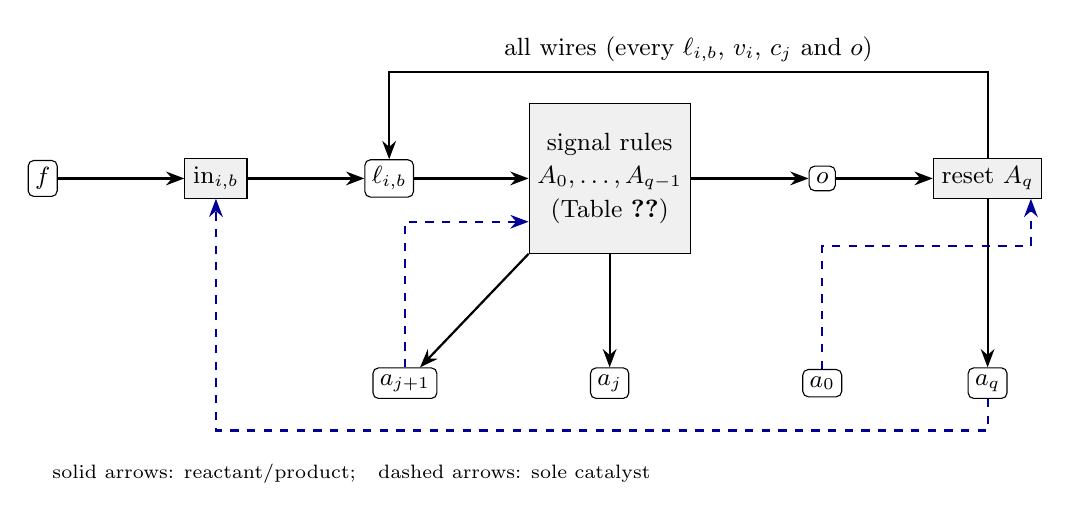
\begin{tikzpicture}[>=Stealth, font=\small,
  mol/.style={draw,rounded corners=2pt,inner sep=2.5pt,fill=white},
  rxn/.style={draw,fill=black!6,inner sep=3pt},
  flow/.style={->,thick},
  cat/.style={->,thick,dashed,blue!60!black}]
 % food and inputs
 \node[mol] (f) at (0,0) {$f$};
 \node[rxn] (in) at (2.2,0) {$\mathrm{in}_{i,b}$};
 \node[mol] (l) at (4.4,0) {$\ell_{i,b}$};
 \draw[flow] (f) -- (in);
 \draw[flow] (in) -- (l);
 % rules
 \node[rxn,minimum height=1.9cm,align=center] (rules) at (7.2,0) {signal rules\\[1pt]$A_0,\dots,A_{q-1}$\\[1pt](Table~\ref{tab:rules})};
 \draw[flow] (l) -- (rules);
 \node[mol] (o) at (9.9,0) {$o$};
 \draw[flow] (rules) -- (o);
 % reset
 \node[rxn] (reset) at (12.0,0) {reset $A_q$};
 \draw[flow] (o) -- (reset);
 \draw[flow] (reset.north) |- (4.4,1.35) node[pos=0.75,above]{all wires (every $\ell_{i,b}$, $v_i$, $c_j$ and $o$)} -- (l.north);
 % markers and catalysis cycle
 \node[mol] (aq) at (12.0,-2.6) {$a_q$};
 \node[mol] (a0) at (9.9,-2.6) {$a_0$};
 \node[mol] (aj) at (7.2,-2.6) {$a_{j}$};
 \node[mol] (aj1) at (4.6,-2.6) {$a_{j+1}$};
 \draw[flow] (reset.south) -- (aq);
 \draw[flow] (rules.south) -- (aj);
 \draw[flow] (rules.south west) -- (aj1);
 \draw[cat] (aq.south) |- (2.2,-3.2) -- (in.south);
 \draw[cat] (a0.north) |- ($(reset.south)+(0.55,-0.6)$) -- ($(reset.south)+(0.55,0)$);
 \draw[cat] (aj1.north) |- ($(rules.west)+(0,-0.55)$);
 \node[align=left,anchor=west,font=\scriptsize] at (0,-3.75) {solid arrows: reactant/product;\quad dashed arrows: sole catalyst};
\end{tikzpicture}
\caption{Schematic of $Q_\varphi$. Input reactions turn food into literal wires; the signal rules derive $o$ exactly when $H_\varphi$ accepts the selected choices; the reset turns $o$ into every wire. Each reaction $A_j$ produces its own marker $a_j$ and is catalysed only by $a_{j+1}$ (indices modulo $q+1$), and the input reactions are catalysed only by $a_q$; this single catalytic cycle forces every auxiliary reaction into every RAF.}
\label{fig:source}
\end{figure}

\subsection{Exact RAF normal form}

\begin{lemma}[Mandatory cycle]\label{lem:cycle}
Every RAF of $Q_\varphi$ contains $\cA$, hence equals $S(T)$ for a unique choice set $T$.
\end{lemma}
\begin{proof}
A RAF is nonempty, and each of its reactions needs its unique catalyst marker in the food closure. A marker enters closure only through its unique producer, which must be selected. Thus some $A_j$ is selected; the catalyst condition for $A_j$ forces $A_{j+1 \bmod (q+1)}$, and iterating around the finite cycle forces all of $\cA$. The input reactions are disjoint from $\cA$, so $T$ is unique.
\end{proof}

\begin{lemma}[The reset cannot enable itself]\label{lem:reset}
If $S(T)$ is a RAF then $H_\varphi(T)$ holds.
\end{lemma}
\begin{proof}
Since the reset is selected and $S(T)$ is food-generated, $o\in\cl_{S(T)}(F)$. Consider the first closure stage $i$ at which $o$ appears. At all stages before $i$ the reset is not enabled, so its products contribute nothing, and removing the reset leaves stages $0,\dots,i$ unchanged. Hence $o$ is derivable from the food by $S(T)\setminus\{A_q\}$. Reset-free generation is exactly forward application of the signal rules to the literal wires of $T$, which reaches $o$ if and only if $H_\varphi(T)$.
\end{proof}

An equivalent closed-set argument: if $H_\varphi(T)$ fails, let $W$ consist of food, all reset-free reachable wires, and all markers; $o\notin W$. Every non-reset reaction with reactants in $W$ has products in $W$, and the reset has a reactant outside $W$, so $\cl_{S(T)}(F)\subseteq W$ and the reset is not food-generated. Admitting all markers into $W$ is harmless because catalysts play no role in generation.

\begin{lemma}[Exact normal form]\label{lem:normal}
The RAFs of $Q_\varphi$ are exactly the sets $S(T)$ with $H_\varphi(T)$, and $S(T)\subseteq S(T')$ if and only if $T\subseteq T'$. Consequently
\begin{equation}\label{eq:family}
 \Irr(Q_\varphi)=\{S(P_i):1\le i\le n\}\ \dot\cup\ \{S(T_\alpha):\alpha\models\varphi\},
 \qquad |\Irr(Q_\varphi)|=n+\#\SAT(\varphi).
\end{equation}
\end{lemma}
\begin{proof}
Lemmas~\ref{lem:cycle} and~\ref{lem:reset} give one direction. Conversely, if $H_\varphi(T)$ holds, reset-free derivation reaches $o$, the reset then makes every wire available, every auxiliary reaction has its reactants in closure and produces its marker, and the selected input reactions consume food; all catalysts $a_j$ are in closure, and the set is nonempty since it contains the reset. So $S(T)$ is a RAF. Inclusion of the sets $S(T)$ agrees with inclusion of choice sets because $\cA$ is common and disjoint from the inputs; applying the correspondence to every subset and Lemma~\ref{lem:choices} gives \eqref{eq:family}. The union is disjoint because $|T_\alpha|=n$ and $T_\alpha$ contains no conflict pair, so $T_\alpha\neq P_i$ even when $n=2$.
\end{proof}

Preserving only existence of a RAF would not suffice for what follows; \eqref{eq:family} describes the entire family. The mandatory cycle removes any freedom to realize the same choice set by different auxiliary subsets, which would otherwise change the number and identity of irreducible outputs. The reset is what makes every accepted $S(T)$ food-generated regardless of which branch of $H_\varphi$ holds, and Lemma~\ref{lem:reset} is what prevents the auxiliary cycle from supporting a spurious RAF on its own.

\begin{example}[A worked instance]\label{ex:worked}
Take $n=3$, $m=2$. Then $q=22$, $d_\varphi=36$, $r_\varphi=29$, and the input has $N=3235$ bits. Every output has size $q+1+|T|$. For $\varphi=(x_1)\wedge(\neg x_1)$ there are no satisfying assignments: $\Irr(Q_\varphi)$ consists of the three conflict-pair sets, each of size $25$, and the required output has $B=(29+1)\cdot3+1=91$ bits. For $\varphi=(x_1)\wedge(x_2)$ over the same three-variable universe there are two satisfying assignments: $\Irr(Q_\varphi)$ has five members, three of size $25$ and two of size $26$, and $B=151$. The size-generating polynomial of the family is $n z^{q+3}+\#\SAT(\varphi)\,z^{q+n+1}$; for $n>2$ the satisfying-assignment outputs are strictly larger than the baseline pairs, illustrating that inclusion-minimality is not minimum size.
\end{example}

\subsection{A deadline computable before enumeration}

Let $\cG_0=\{S(P_i):1\le i\le n\}$. By \eqref{eq:family} this is a polynomially constructible family of $n$ distinct irreducible RAFs, and
\begin{equation}\label{eq:baseline}
 \Irr(Q_\varphi)=\cG_0\iff|\Irr(Q_\varphi)|=n\iff\varphi\text{ is unsatisfiable}.
\end{equation}
In the unsatisfiable case the required output length is the known polynomial
\[
 B_0=(r_\varphi+1)\,n+1 .
\]
This is the encoded length of the complete output, not merely a bound on the number of outputs; the formal development bounds it by $20\,|\varphi|^3$ in terms of the encoded length $|\varphi|$ of the formula.

\begin{theorem}[Lower bound]\label{thm:lower}
If a pair $(E,p)$ satisfies the enumeration contract of Section~\ref{sec:contract}, then $\SAT\in\PP$, and hence $\PP=\NP$.
\end{theorem}
\begin{proof}
Given $\varphi$ (padded to $n\ge2$), construct $Q_\varphi$, encode it, compute $T_\varphi=p(N_\varphi+B_0)$, and simulate $E$ for at most $T_\varphi$ transitions. Declare $\varphi$ unsatisfiable if and only if $E$ has halted by the deadline with output count exactly $n$.

If $\varphi$ is unsatisfiable, then by \eqref{eq:baseline} the actual output length is $B_0$, so the contract forces $E$ to halt within $T_\varphi$ steps with count $n$. If $\varphi$ is satisfiable, then $|\Irr(Q_\varphi)|>n$, so a halted output has count larger than $n$, and a run that has not halted by the deadline has already excluded the unsatisfiable case. Both outcomes are classified correctly.

The encoding of $Q_\varphi$ and the number $T_\varphi$ have size polynomial in $|\varphi|$, because the dimensions \eqref{eq:dims} and $B_0$ are polynomial and $p$ is fixed. Since $E$ is a fixed machine, bounded simulation with a clock and inspection of the halted unary count cost polynomial overhead. This is a deterministic polynomial-time decider for SAT; NP-completeness of SAT \cite{cook1971complexity,levin1973universal,karp1972reducibility} gives $\PP=\NP$.
\end{proof}

The argument does not wait for a satisfiable instance's possibly enormous output and makes no assertion about when such runs finish. It requires no way of discovering an unknown enumerator's polynomial; it proves the existential implication that any fixed witnesses $(E,p)$ yield a fixed polynomial SAT decider. The hard small-output instances are the \emph{unsatisfiable} formulas, so the theorem should not be summarized as a consequence of exponentially many outputs. In the formal development the source compiler, the bounded simulator, the clock, the syntax guard and the count test are all machine constructions with proved bounds; none is an assumed oracle.

\section{The conditional upper bound}\label{sec:upper}

Assume $\PP=\NP$ and fix, once and for all, a deterministic polynomial-time SAT decider. Lemma~\ref{lem:cnf} then gives a polynomial-time procedure for $\Avail_Q(\cG,U)$, uniformly in $Q$, $\cG$ and $U$.

\medskip
\noindent\textbf{Procedure.} Start with $\cG=\varnothing$ and repeat: query $\Avail_Q(\cG,R)$; if false, stop. Otherwise set $U=R$ and scan the reactions once in their fixed input order; for each $a$, replace $U$ by $U\setminus\{a\}$ if $\Avail_Q(\cG,U\setminus\{a\})$ holds. After the scan append $U$ to $\cG$. On termination write the unary count $|\cG|$ and the stored masks in the format \eqref{eq:output}.

\begin{lemma}[Filtered deletion]\label{lem:sweep}
If a round starts with $\cG\subseteq\Irr(Q)$ and $\Avail_Q(\cG,R)$ true, its deletion scan ends at a set $U\in\Irr(Q)\setminus\cG$.
\end{lemma}
\begin{proof}
$\Avail_Q(\cG,U)$ remains true after every accepted deletion. If deleting $a$ is rejected, the container without $a$ has no avoiding witness; later containers only shrink, so by monotonicity the deletion of $a$ never becomes feasible. Hence the final $U$ is a minimal container satisfying $\Avail_Q(\cG,\cdot)$: any proper subset omits some retained $a$ and lies inside the failed container $U\setminus\{a\}$.

Let $S\subseteq U$ be an avoiding RAF witnessing the final query. $S$ is itself a feasible container, so $S=U$ by minimality; thus $U$ is a RAF. If a proper RAF subset $V\subsetneq U$ existed it would still avoid all of $\cG$ (an $I\subseteq V\subseteq U$ would contradict avoidance of $U$), so $V$ would be a smaller feasible container. Hence $U\in\Irr(Q)$. Finally $U\notin\cG$, since otherwise avoidance would require $U\nsubseteq U$.
\end{proof}

\begin{theorem}[Conditional upper bound]\label{thm:upper}
If $\PP=\NP$, there exist a fixed deterministic multitape machine $E$ and a polynomial $p$ satisfying the enumeration contract of Section~\ref{sec:contract}.
\end{theorem}
\begin{proof}
By Lemma~\ref{lem:sweep} and induction, the stored list is duplicate-free, consists of irreducible RAFs, and grows by one in every successful round. There are exactly $K=|\Irr(Q)|$ successful rounds followed by one negative query, at which point Lemma~\ref{lem:completion} certifies completeness. The case $K=0$ never enters a minimization round.

For the time bound set $W=N+B$. At every stage $g=|\cG|\le K$, the stored masks and exclusion clauses have length polynomial in $N+gr\le W$, and Lemma~\ref{lem:cnf} bounds each query's encoding by a polynomial in $W$; composing with the fixed SAT decider gives a fixed polynomial per query. Each successful round makes at most $r+1$ queries and the final round one, so the number of queries is at most $(r+1)K+1\le W+1$. Constructing the queries, scanning masks, updating the stored family, and writing the final count and masks add polynomial overhead. Hence the total time is bounded by a polynomial in $W$ that depends only on the chosen SAT decider.
\end{proof}

The filter must stay in force \emph{during} minimization. Minimizing an arbitrary RAF from the full reaction set could return a known output and stall progress; in the procedure above every accepted container retains a witness that avoids all known outputs. Theorems~\ref{thm:lower} and~\ref{thm:upper} together prove Theorem~\ref{thm:main}.

\section{Consequences}\label{sec:consequences}

The results of this section are conventional deductions from the exact correspondence \eqref{eq:family} and the verified finite semantics; their complexity-class statements have not separately been compiled in Lean (Section~\ref{sec:formal} states precisely what has).

\subsection{Certification and counting}

Let $\Exact(Q,\cG)$ mean that a supplied explicit family $\cG$ of reaction masks consists of exactly all irreducible RAFs of $Q$ (repeated masks are deduplicated first), and let $\Extra(Q,\cG)$ mean that $\cG\subseteq\Irr(Q)$ and $\Irr(Q)\setminus\cG\neq\varnothing$. Input size includes $Q$ and all supplied masks.

\begin{proposition}[Certification]\label{prop:conp}
$\Exact$ is $\coNP$-complete, and $\Extra$ is $\NP$-complete, under polynomial many-one reductions. Hardness holds already for systems with one food molecule and one catalyst per reaction.
\end{proposition}
\begin{proof}
Validity of each supplied mask is polynomial by Lemma~\ref{lem:irrtest}. If all members are valid, an avoiding RAF is a polynomial-size certificate that $\cG$ is incomplete (Lemma~\ref{lem:completion}), so $\Extra\in\NP$ and $\Exact\in\coNP$ (accept the complement when validity fails or an avoiding RAF exists). For hardness, map $\varphi$ to $(Q_\varphi,\cG_0)$: by \eqref{eq:baseline} the family is complete exactly when $\varphi$ is unsatisfiable, and $\cG_0$ is always valid, so the reduction lands in the valid part for $\Extra$ as well.
\end{proof}

Consequently, unless $\NP=\coNP$, complete families do not in general admit polynomial-size certificates checkable in polynomial time; this does not exclude short certificates on particular instances, and the deletion criterion of \cite{steel2013minimal} is exactly such a certificate when the product of the list sizes is small. The parameterized refinement with $|\cG|$ as parameter is co-$\mathrm{W[P]}$-complete \cite{certification2026}; that is a separate result and is not a consequence of Proposition~\ref{prop:conp}.

\begin{proposition}[Counting]\label{prop:counting}
The function $Q\mapsto|\Irr(Q)|$ is in $\sharpP$ and is $\sharpP$-hard under polynomial-time Turing reductions; hence it is $\sharpP$-complete in that sense.
\end{proposition}
\begin{proof}
Membership: guess a width-$r$ mask and accept exactly when Lemma~\ref{lem:irrtest} holds; each output corresponds to one accepted mask, not to its support certificates. Hardness: by \eqref{eq:family}, $\#\SAT(\varphi)=|\Irr(Q_\varphi)|-n$ for $\varphi$ with $n\ge2$ declared variables; if padding added $u$ variables, divide by $2^u$. Counting satisfying assignments is $\sharpP$-complete \cite{valiant1979complexity}.
\end{proof}

The reduction is not parsimonious: it deliberately adds $n$ baseline outputs. Note also that output-polynomial enumeration, even under $\PP=\NP$, is not a polynomial-time counter, because its running time may still be exponential in the input through the output length.

\subsection{Polynomial delay}

The contract of Section~\ref{sec:contract} writes the count first. Under the usual convention in which outputs are streamed as records, the classification persists.

\begin{proposition}[Streaming enumeration]\label{prop:delay}
Irreducible RAFs admit a polynomial-delay, polynomial-space enumeration algorithm if and only if $\PP=\NP$.
\end{proposition}
\begin{proof}
Assume $\PP=\NP$. For a partial mask $\sigma\in\{0,1\}^{\le r}$ (a decision on the first $|\sigma|$ reactions) the language ``some $I\in\Irr(Q)$ extends $\sigma$'' is in $\NP$, since a full mask can be guessed and checked by Lemma~\ref{lem:irrtest}; fix a polynomial-time decider for it. Traverse the binary prefix tree depth first, entering only prefixes with a valid extension. The depth is $r$, so between consecutive output leaves, and before the first or after the last, at most $O(r)$ extension tests are made; the traversal stores only the current path. This is the standard extension-oracle route to bounded delay \cite[Section~4]{strozecki2023enumeration}. Conversely, a polynomial-delay enumerator has total time polynomial in $N$ plus the number of records; buffering its masks and prefixing the unary count yields a machine satisfying the contract of Section~\ref{sec:contract}, and Theorem~\ref{thm:lower} gives $\PP=\NP$.
\end{proof}

\subsection{Deletion survival and essential reactions}

\begin{proposition}[Survival under deletion]\label{prop:survival}
For every $D\subseteq R$,
\[
 \maxRAF_Q(R\setminus D)\neq\varnothing\iff\exists I\in\Irr(Q):\ I\cap D=\varnothing .
\]
Hence the inclusion-minimal RAF-destroying deletion sets are exactly the minimal transversals of $\Irr(Q)$.
\end{proposition}
\begin{proof}
A surviving RAF contains an irreducible one, which is disjoint from $D$; a surviving irreducible RAF is itself a witness.
\end{proof}

A partial family thus gives a one-sided certificate: an unhit listed member proves survival, while hitting every listed member proves extinction only if the list is complete or a residual maxRAF test confirms it.

\begin{proposition}[Universally required reactions]\label{prop:essential}
If $Q$ contains a RAF, then for every $a\in R$,
\[
 a\in\bigcap_{I\in\Irr(Q)}I\iff\maxRAF_Q(R\setminus\{a\})=\varnothing .
\]
The intersection of all irreducible RAFs is therefore computable with $r$ maxRAF calls and no enumeration.
\end{proposition}
\begin{proof}
Apply Proposition~\ref{prop:survival} with $D=\{a\}$.
\end{proof}

Such indispensable reactions already appear in the lower-bound method of \cite[Section~5]{steel2013minimal}; Proposition~\ref{prop:essential} is their exact family interpretation. When no RAF exists the family is empty and the vacuous intersection should be reported as ``no RAF'', not as essentiality. The complete family does not reconstruct every surviving reaction: with $a\colon f\to x$ and $b\colon x\to y$ both catalysed by food $f$, the unique irreducible RAF is $\{a\}$ while the maxRAF is $\{a,b\}$, so $\bigcup\Irr(Q)$ need not equal $\maxRAF_Q(R)$, and the family determines survival but not the residual maxRAF or its size.

\subsection{Structural indicators that cannot detect hardness}

\begin{proposition}[Overlap and low-order deletion response]\label{prop:indicators}
Let $\varphi$ have $n\ge2$ variables and let $Q_\varphi$ be as in Construction~\ref{con:source}, with $a=|\cA|=q+1$.
\begin{enumerate}[label=\textup{(\alph*)}]
\item Any two members of $\Irr(Q_\varphi)$ have Jaccard similarity at least $a/(a+2n)$. Adding tautological clauses to $\varphi$ leaves $\#\SAT(\varphi)$ unchanged while increasing $a$, so for fixed $n$ this bound tends to $1$ along a family of instances whose completion problem remains NP-hard.
\item Let $D$ consist of input reactions only. If $|D|<n$ then $\maxRAF_{Q_\varphi}(R_\varphi\setminus D)=R_\varphi\setminus D$, independently of $\varphi$. If $D$ deletes exactly one input of every conflict pair, leaving the choice set of an assignment $\alpha$, then $\maxRAF_{Q_\varphi}(R_\varphi\setminus D)$ is $R_\varphi\setminus D$ if $\alpha\models\varphi$ and $\varnothing$ otherwise.
\end{enumerate}
\end{proposition}
\begin{proof}
(a) Members share $\cA$ and differ in at most $2n$ input reactions. (b) If fewer than $n$ inputs are deleted, some conflict pair survives intact, the remaining choice set is accepted, and by Lemma~\ref{lem:normal} the whole remaining canonical set is a RAF. If exactly one input of every pair is deleted, the surviving choice set $T_\alpha$ is conflict-free, so it and its proper subsets are accepted only if $\alpha\models\varphi$; the maxRAF is then the whole remaining set or empty by \eqref{eq:family}.
\end{proof}

Thus the SAT distinction can first appear at cooperative deletion order $n$ while all lower-order input-deletion responses are identical, and pairwise output overlap can be arbitrarily close to one. These are limitations of proposed structural indicators, not claims about typical chemical networks.

\subsection{Positive and negative frontiers}\label{sec:frontier}

By Proposition~\ref{prop:survival} the negative frontier of the monotone viability predicate is the minimal transversal family of $\Irr(Q)$, and it need not be compact. For $k$ independent two-reaction catalytic cycles, each consuming food and producing its partner's catalyst, the irreducible RAFs are the $k$ pairs, and a minimal destructive deletion chooses one reaction from each pair: there are $2^k$ of them. An enumeration algorithm charged only for its $k$ positive outputs therefore cannot be required to materialize the negative frontier. This is also why Theorem~\ref{thm:main} says nothing about the explicit transversal-hypergraph problem \cite{fredman1996complexity,eiter1995identifying,mary2024enumeration}: a catalytic reaction system supplies a compact polynomial-time viability oracle, not a small explicit hypergraph whose transversals are its irreducible RAFs, and the distinction between learning both boundaries and recovering only the positive one is the one drawn in \cite{bioch1995complexity}.

\section{Formal verification}\label{sec:formal}

\subsection{The exported theorem}

The classification is realized in Lean~4 (toolchain \texttt{v4.30.0}, with a pinned \texttt{mathlib} revision) by the declaration
\begin{quote}\raggedright\ttfamily\small
IrrRAFEnumeration.outputPolynomialEnumeration\_iff\_P\_eq\_NP :\\
\quad EnumerationContract.OutputPolynomialEnumeration $\leftrightarrow$ Complexity.P = Complexity.NP
\end{quote}
in \lean{proofs/IrrRAFEnumeration/Classification.lean}, assembled from the two directions:
\begin{small}\begin{verbatim}
theorem outputPolynomialEnumeration_of_P_eq_NP
    (h : Complexity.P = Complexity.NP) : OutputPolynomialEnumeration := by
  exact outputPolynomialEnumeration_of_initializer h
    (fun k => <24, originalInitializerTM k, originalInitializerPolynomial,
      originalInitializer_correct k>)
    (fun _ E p hE => enumerates_of_finEnumerates E p hE)

theorem outputPolynomialEnumeration_iff_P_eq_NP :
    EnumerationContract.OutputPolynomialEnumeration <->
      Complexity.P = Complexity.NP :=
  <P_eq_NP_of_outputPolynomialEnumeration, outputPolynomialEnumeration_of_P_eq_NP>
\end{verbatim}\end{small}
(angle brackets stand for Lean's anonymous-constructor brackets). The theorem has no outer parameters or hypotheses. Its recorded axiom dependencies are \lean{propext}, \lean{Classical.choice} and \lean{Quot.sound} only; there is no \lean{sorry} and no additional mathematical axiom.

The left-hand side is the literal contract of Section~\ref{sec:contract}:
\begin{small}\begin{verbatim}
def Enumerates {k : Nat} (E : TM k) (p : Polynomial Nat) : Prop :=
  forall (M R : Type) [DecidableEq M] [DecidableEq R] [Fintype R]
    (a b : Nat) (em : M ~= Fin a) (er : R ~= Fin b)
    (Q : CRS M R) (C : Catalysis M R) [DecidableRel C],
    exists (rows : List (Finset R)) (c : Cfg k E.Q) (t : Nat),
      rows.Nodup /\ rows.toFinset = irrRAFFamily Q C /\
      t <= p.eval ((inputBits Q C em er).length
                  + (outputBits er rows).length) /\
      E.reachesIn t (E.initCfg (inputBits Q C em er)) c /\ E.halted c /\
      c.output.HasOutput (outputBits er rows)

def OutputPolynomialEnumeration : Prop :=
  exists (k : Nat) (E : TM k) (p : Polynomial Nat), Enumerates E p
\end{verbatim}\end{small}
Here \lean{inputBits} is \eqref{eq:input}, \lean{outputBits} is \eqref{eq:output} with the proved length identity $(r+1)K+1$, \lean{irrRAFFamily Q C} is the finite set of inclusion-minimal nonempty RAFs, and the quantification ranges over all finite types $M$, $R$ with explicit bijections to initial segments of $\Nat$. The right-hand side uses the machine-based classes $\PP=\bigcup_k\mathrm{DTIME}(n^k)$ and $\NP=\bigcup_k\mathrm{NTIME}(n^k)$ of \texttt{complexitylib} \cite{schlesinger2025complexitylib}, from which the development also imports the Cook--Levin theorem \lean{SAT.NPComplete_language}. That library is vendored at an immutable commit with its Apache-2.0 notices; its declarations are unchanged and are compiled locally.

\subsection{Concordance}

Table~\ref{tab:concordance} maps the statements of this paper to the Lean declarations that realize them. All paths are relative to \lean{proofs/IrrRAFEnumeration/}.

\begin{table}[htbp]
\centering\small
\begin{tabular}{>{\raggedright\arraybackslash}p{0.26\linewidth}>{\raggedright\arraybackslash}p{0.67\linewidth}}
\toprule
Paper statement & Lean declaration(s)\\
\midrule
Theorem~\ref{thm:main} & \lean{Classification.lean}: \lean{outputPolynomialEnumeration_iff_P_eq_NP}\\
Encoding, Definition~\ref{def:encoding} & \lean{EnumerationContract.lean}: \lean{inputBits}, \lean{outputBits}, \lean{outputBits_length}, \lean{Enumerates}, \lean{OutputPolynomialEnumeration}\\
RAF semantics, Definition~\ref{def:raf} & \lean{proofs/RAF/Core/Closure.lean}, \lean{proofs/RAF/Core/RAF.lean}; \lean{RAFCompletion.lean}: \lean{mem_irrRAFFamily}, \lean{hasRAFWithin_iff_contains_irrRAF}\\
Lemma~\ref{lem:completion} & \lean{PositiveCompletion.lean}: \lean{available_univ_iff_missing}, \lean{available_mono}\\
Lemma~\ref{lem:cnf} & \lean{PositiveSupportedTrace.lean}: \lean{isRAF_iff_supported}; \lean{PositiveCompletionCNF.lean}: \lean{formula_eval_iff}, \lean{formula_sound}; \lean{PositiveCompletionReduction.lean}: \lean{formula_complete}, \lean{formula_satisfiable_iff}\\
Lemma~\ref{lem:choices} & \lean{SATCompletion.lean}: \lean{minimal_eval_iff} (hypothesis $n\ge2$)\\
Lemma~\ref{lem:cycle} & \lean{CircuitSource.lean}: \lean{raf_contains_all_aux}\\
Lemma~\ref{lem:reset} & \lean{CircuitClosure.lean}: \lean{raf_output_reached_without_reset}, \lean{isRAF_iff_all_aux_and_output}\\
Lemma~\ref{lem:normal}, eq.~\eqref{eq:family} & \lean{CircuitBijection.lean}: \lean{canonical_irreducible_iff}; \lean{SATSource.lean}: \lean{accepts_encode_iff_eval}; \lean{SATReduction.lean}: \lean{sourceSet_irreducible_iff}, \lean{irreducible_iff_exists_sourceSet}\\
Eq.~\eqref{eq:baseline}, length $B_0$ & \lean{SATFamily.lean}: \lean{baseline_card}, \lean{baseline_subset_irrRAFFamily}, \lean{irrRAFFamily_eq_baseline_iff_unsat}; \lean{SATCountTimeout.lean}: \lean{irrRAFFamily_card_eq_iff_cnf_unsat}, \lean{countTimeout_length_polynomial}, \lean{bounded_count_decides_cnf_unsat}\\
Theorem~\ref{thm:lower} & \lean{SourceEnumeratorRun.lean}: \lean{source_enumerator_no_case}; \lean{SATMembership.lean}: \lean{SAT_mem_P_of_sourceCountBound}; \lean{NegativeClassification.lean}: \lean{P_eq_NP_of_outputPolynomialEnumeration}\\
Lemma~\ref{lem:sweep} & \lean{PositiveCompletion.lean}: \lean{sweep_minimal}, \lean{minimal_available}, \lean{sweep_new_minimal}, \lean{raf_sweep_new}\\
Theorem~\ref{thm:upper}, prepared machine & \lean{CompletionUniformEnumerationCost.lean}: \lean{preparedEnumeration_polynomial}; \lean{CompletionConditionalEnumeration.lean}: \lean{preparedEnumeration_of_P_eq_NP}\\
Original-input initializer & \lean{CompletionOriginalInput.lean}: \lean{originalInitializer_correct}, \lean{initialFinalWork_eq}\\
Arbitrary identifiers & \lean{CompletionLabelTransport.lean}: \lean{enumerates_of_finEnumerates}\\
Theorem~\ref{thm:upper}, composed & \lean{Classification.lean}: \lean{outputPolynomialEnumeration_of_P_eq_NP}\\
\bottomrule
\end{tabular}
\caption{Concordance between the paper and the Lean development.}
\label{tab:concordance}
\end{table}

\subsection{From prepared computation to the original input}

The conditional direction first obtains, from $\PP=\NP$, one SAT machine and one polynomial \emph{before} quantifying over the system. Its prepared enumeration routine maintains the base chemistry formula, the accumulated exclusion clauses, the current container mask, the minimization state, the stored output masks and the output count; a successful round appends a new mask and its exclusion clause together, and the final writer realizes the count-first format. This routine has one uniform polynomial bound $p_1(N+B)$.

A separate initializer starts from the actual encoded input, reads the dimensions, constructs the chemistry CNF, installs the full reaction mask and counters, and establishes the exact entry configuration of the prepared routine on the physical tapes and head positions. Its proved bound is
\begin{equation}\label{eq:init}
 p_0(N)=50\,000\,000\,(N+1)^6+6N^2+21N+54 ,
\end{equation}
a conservative execution bound rather than a suggested implementation cost. Retained compiler scratch occupies a disjoint bank of work tapes that the prepared routine never reads. Sequential composition gives
\[
 p_0(N)+1+p_1(N+B)\le(p_0+p_1+1)(N+B),
\]
using nonnegative coefficients and $N\le N+B$, so initialization is charged on the original input and leaves no prepared-formula premise in the root theorem.

The finite-index proof is transported through the supplied molecule and reaction bijections: closure stages, catalyst availability, RAF status and minimality are preserved, and the input bits and output masks are identical under the change of interpretation. The same machine run therefore serves arbitrary finite identifiers with no uncharged conversion, and distinct reactions with identical incidence data remain distinct.

\subsection{Trust boundary}

Strict verification in the frozen environment accepted the root with warnings treated as errors. The receipt records the toolchain \texttt{leanprover/lean4:v4.30.0}, the SHA-256 of the pinned dependency manifest (\texttt{a8df0b60\ldots}), of the root source (\texttt{3aee5560\ldots}) and of the compiled root artifact (\texttt{1bbc72c4\ldots}), and an elapsed time of $66.3$ seconds for the final module; a subsequent audit rehashed the root and all $378$ recorded local source/artifact dependency pairs. Full hashes and the verification command are in Appendix~\ref{app:repro}.

What is trusted: the Lean~4 kernel and the pinned \texttt{mathlib} and \texttt{complexitylib} revisions, including the latter's Turing-machine model and its definitions of $\PP$, $\NP$ and SAT. What is proved: everything in Table~\ref{tab:concordance}, for concrete machines and actual tape contents. What is \emph{not} proved in Lean: the complexity-class statements of Section~\ref{sec:consequences} (conventional proofs from verified finite lemmas), and any property of the reference software of Section~\ref{sec:practice}, which is not extracted from the development. Neither a solver experiment nor a numerical audit is a premise of Theorem~\ref{thm:main}.

\section{A practical enumerator and a bounded pilot}\label{sec:practice}

The formal upper bound needs only a SAT \emph{decider}. A practical solver returns a model, which yields an avoiding RAF at once and can be minimized by ordinary maxRAF calls instead of further SAT queries.

\medskip
\noindent\textbf{Model-assisted enumeration.} Maintain a validated duplicate-free known family $\cG$ (initially empty or user-supplied) and the base formula $\Psi(Q,\varnothing,R)$ with one exclusion clause \eqref{eq:cnf7} per member of $\cG$. Repeat: solve. If unsatisfiable, return $\cG$ as complete. If a model is returned, let $S$ be its selected set, verify independently that $S$ is a RAF avoiding $\cG$, then scan reactions in fixed order and, for each $a\in T$ (initially $T=S$), replace $T$ by $\maxRAF_Q(T\setminus\{a\})$ whenever that is nonempty. Verify irreducibility of the final $T$ by Lemma~\ref{lem:irrtest}, emit it, add its exclusion clause, and continue. If the solver reports unknown or a resource limit is hit, return $\cG$ with status \emph{incomplete}.

\begin{proposition}[Solver-call count]\label{prop:calls}
Every set emitted by the model-assisted procedure is a new irreducible RAF, and no output is repeated. If $|\Irr(Q)|=K$ and $g$ distinct valid members were supplied initially, a completed uninterrupted run makes exactly $K-g+1$ solver calls ($K-g$ satisfiable, one final unsatisfiable) and at most $r(K-g)$ maxRAF calls during minimization.
\end{proposition}
\begin{proof}
Every intermediate $T$ is a RAF contained in the avoiding witness $S$, so it remains avoiding by heredity. If deleting $a$ leaves no RAF, subsequent shrinkage cannot change that, so one pass suffices and the final $T$ is irreducible and new, as in Lemma~\ref{lem:sweep}. Adding $\bigvee_{a\in T}\neg s_a$ excludes exactly the supersets of $T$, which contain no other irreducible RAF by the antichain property, so every missing output stays reachable. Each satisfiable call therefore enlarges $\cG$ by one distinct member, and the count follows.
\end{proof}

This is a count of solver invocations, not a running-time guarantee: the calls can be hard, as Theorem~\ref{thm:lower} shows they must sometimes be. Sampling can populate the initial family cheaply, after which one completion query settles whether anything was missed; this combines fast discovery with an exact stopping condition without making the sampler uniform. Compared with the tuple-deletion criterion \eqref{eq:tuple}, the SAT formulation expresses the choices and the chemical witness jointly instead of materializing the Cartesian product $I_1\times\cdots\times I_g$.

\medskip
\noindent\textbf{A bounded pilot.} A small Python reference implementation of this procedure over Z3 \cite{demoura2008z3} was run on toy fixtures to check the semantics and the call-count identity, with every emitted mask re-checked by independent closure and single-deletion maxRAF tests. The fixtures are ligation-only polymer systems over binary strings of length at most $n\in\{2,3\}$ with food $\{0,1\}$ and independent catalyst assignments with probability $0.22$ (three construction seeds each), and one published example network from Hordijk's RAF repository with each reversible reaction split into two separately selectable directions. Table~\ref{tab:pilot} shows the $n=3$ instances and the published example. On every completed run from an empty family the model-assisted variant made exactly $K+1$ solver calls; the decision-only variant, which minimizes by further SAT queries as in Section~\ref{sec:upper}, made many more (for the seven-core instance, $8$ versus $148$) and all complete methods agreed on the family. On the $392$-reaction published example the unoptimized reference code exhausted its four-second budget while still \emph{building} the formula, before any solver call, and reported unknown; sampling found three verified cores per seed and no completeness statement. These are single-run pilot measurements of an unoptimized script, intended to validate semantics and the identity of Proposition~\ref{prop:calls}, not a performance study and not a comparison with the optimized implementations of \cite{hordijk2015algorithms,hordijk2026enumerating}.

\begin{table}[htbp]
\centering\small
\begin{tabular}{llllrrr}
\toprule
Instance & $d/r$ & Method & Status & $|\cG|$ & SAT & maxRAF\\
\midrule
polymer $n{=}3$, seed 11 & $14/20$ & model-assisted & complete & 4 & 5 & 10\\
 & & decision-only & complete & 4 & 85 & 0\\
 & & exhaustive & complete & 4 & 0 & 0\\
polymer $n{=}3$, seed 23 & $14/20$ & model-assisted & complete & 2 & 3 & 5\\
 & & decision-only & complete & 2 & 43 & 0\\
 & & exhaustive & unknown & 2 & 0 & 0\\
polymer $n{=}3$, seed 47 & $14/20$ & model-assisted & complete & 7 & 8 & 38\\
 & & decision-only & complete & 7 & 148 & 0\\
 & & exhaustive & complete & 7 & 0 & 0\\
 & & sampling, 3 seeds & unknown & 6, 7, 7 & 0 & $\approx2550$\\
published example, split & $62/392$ & model-assisted & unknown & 0 & 0 & 0\\
 & & sampling, 3 seeds & unknown & 3, 3, 3 & 0 & $\approx2980$\\
\bottomrule
\end{tabular}
\caption{Bounded pilot with a four-second budget per run. $|\cG|$ is the number of independently verified outputs; ``SAT'' and ``maxRAF'' count solver and maxRAF calls, the latter excluding output validation. ``Unknown'' means the budget expired without a completeness certificate.}
\label{tab:pilot}
\end{table}

\section{Discussion}\label{sec:discussion}

\subsection{What the classification says for applications}

RAF analysis has been applied to metabolic reconstructions such as the \emph{E.~coli} network \cite{sousa2015ecoli} and to origin-of-metabolism questions \cite{xavier2020autocatalytic}. In that setting Theorem~\ref{thm:main} separates two tasks that are easily conflated: \emph{discovering} minimal structural cores, which sampling and deletion sweeps do efficiently, and \emph{establishing that none remain}, which in the worst case is a SAT problem. The practical recommendation is to report discovered cores together with their completion status, and to use a completion query (Section~\ref{sec:completion}) when an exhaustive conclusion matters. Several structural questions do not require enumeration at all: whether any RAF survives a deletion (Proposition~\ref{prop:survival}, one maxRAF call), and which reactions are required by every irreducible RAF (Proposition~\ref{prop:essential}, $r$ calls).

The object is a finite incidence model with explicit food and catalyst data. Structural survival and essentiality are combinatorial properties of that model, not measurements of gene or organism essentiality, kinetic frequency, mass balance, thermodynamic feasibility or sustained growth; flux-balance and hyperflow formalisms encode distinctions that incidence-only RAFs do not \cite{orth2010flux,andersen2021defining}, and the relationship between RAFs and chemical organizations is its own subject \cite{hordijk2018organizations}. Modelling conventions change the family: splitting a reversible reaction into two selectable directions changes the choice space rather than merely relabelling it, and the identity policy for duplicate reactions or isoenzymes must be declared. Since $\bigcup\Irr(Q)$ can omit reactions of the maxRAF, screening only minimal cores through a downstream quantitative test can miss useful larger RAFs; a combined notion of minimality needs its own search and minimality guarantees.

\subsection{What the classification does not say}

Theorem~\ref{thm:main} does not decide $\PP$ versus $\NP$, does not give an unconditional exponential lower bound, does not exclude useful heuristics or efficient restricted classes, and says nothing about average-case or randomized enumeration. The source uses one food molecule and one catalyst per reaction, so hardness holds under those restrictions, but its finish and reset reactions have unbounded arity; bounded-arity hardness is not established by this construction. The tractable models of \cite{steel2018tractable} are a natural place to look for restricted classes with efficient complete enumeration, provided the restriction is stated on the full reaction model rather than inferred from catalytic topology alone, since Proposition~\ref{prop:indicators} shows that overlap statistics and low-order deletion responses cannot detect the interacting choices.

\subsection{Open problems}

\begin{enumerate}
\item \textbf{Bounded arity.} Is complete enumeration still hard when every reaction has at most two reactants and one product, as in the Set Cover source of \cite{minraf2026}? The reset and finish reactions would have to be replaced by chains whose intermediate products do not create new irreducible RAFs.
\item \textbf{Restricted classes.} For which structurally defined classes (elementary systems, bounded catalytic in-degree, bounded treewidth of the incidence hypergraph) does $\Irr(Q)$ admit polynomial-delay enumeration unconditionally?
\item \textbf{Parameterized delay.} The certification problem is co-$\mathrm{W[P]}$-complete in the list length \cite{certification2026}. Is there a natural parameter, such as the maximum size of an irreducible RAF or the number of reactions with several catalysts, under which enumeration becomes fixed-parameter tractable with polynomial delay?
\item \textbf{Certificates of completeness.} Proposition~\ref{prop:conp} rules out short certificates in general unless $\NP=\coNP$. Which instance classes admit checkable completeness certificates, for example resolution refutations of $\Psi(Q,\Irr(Q),R)$ of polynomial size?
\end{enumerate}

\appendix

\section{Exact formula sizes and the worked example}\label{app:counts}

For implementation planning, let $A_\rho=\sum_a|\rho(a)|$, $A_\pi=\sum_a|\pi(a)|$, $A_C=|C|$, $h=|F|$, $t=|R\setminus U|$ and $H_\cG=\sum_{I\in\cG}|I|$, with $g=|\cG|$. The displayed construction $\Psi(Q,\cG,U)$ has
\[
 v=r+d(d+1)+dr\ \text{ variables},\qquad
 c=1+t+(d-h)+dr+dA_\rho+d^2+A_\rho+r+g\ \text{ clauses},
\]
and, before duplicate removal or simplification,
\[
 \lambda=2r+t+(d-h)+2dr+2(d+1)A_\rho+2d^2+dA_\pi+A_C+H_\cG
\]
literal occurrences. These count the rows of \eqref{eq:cnf1}--\eqref{eq:cnf7}; empty clauses contribute zero literals but count as clauses. For $r=0$ the nonemptiness clause is empty and the formula is unsatisfiable; for $d=0$ no catalyst exists and the catalyst clauses exclude all selections; a reaction with no reactants is enabled at once but still needs a catalyst.

For Example~\ref{ex:worked} the dimension arithmetic is $q=3\cdot3+2\cdot3\cdot2+1=22$, $d_\varphi=6\cdot3+12+2+4=36$, $r_\varphi=15+12+2=29$, $N=2\cdot36+29+2+3\cdot36\cdot29=3235$, $B_0=30\cdot3+1=91$, and for two satisfying assignments $B=30\cdot5+1=151$. A conflict-pair output has $q+1+2=25$ reactions; a satisfying-assignment output has $q+1+n=26$.

\section{Reproduction}\label{app:repro}

The Lean development lives in the repository directory \lean{proofs/IrrRAFEnumeration/} with the RAF core in \lean{proofs/RAF/Core/} and the vendored complexity library in \lean{proofs/Complexitylib/} (upstream commit \texttt{43d4bb1a30bd9384\allowbreak 6eab5480bec8a371\allowbreak 13586109}). The root was verified with the repository's strict bridge, which enters the frozen \texttt{mathlib4\_project} environment and compiles with \texttt{-DwarningAsError=true}:
\begin{small}\begin{verbatim}
python scripts/verify_proof.py proofs/IrrRAFEnumeration/Classification.lean \
  --declaration IrrRAFEnumeration.outputPolynomialEnumeration_iff_P_eq_NP \
  --declaration IrrRAFEnumeration.outputPolynomialEnumeration_of_P_eq_NP \
  --timeout 600 --output classification.verify.json
\end{verbatim}\end{small}
The successful receipt records the following.

\begin{center}\small
\begin{tabular}{@{}ll@{}}
\toprule
Toolchain & \texttt{leanprover/lean4:v4.30.0}\\
\texttt{mathlib} revision & \texttt{c5ea00351c28e24afc9f0f84379aa41082b1188f}\\
Dependency manifest SHA-256 & \texttt{a8df0b606ec258561c226df89856884b}\\
 & \texttt{e433c19b49fb0a27335d69bb2b6e9fac}\\
Root source SHA-256 & \texttt{3aee5560a7b19cdd7f2d2ef5e5806989}\\
 & \texttt{fe0758a8b899f780821d4d5aadd0d473}\\
Root artifact SHA-256 & \texttt{1bbc72c4bf4b5b44a23ee9aab87014f9}\\
 & \texttt{85f4c007160c796e0ef307b455d2925c}\\
Exported theorems & \texttt{outputPolynomialEnumeration\_iff\_P\_eq\_NP}\\
 & \texttt{outputPolynomialEnumeration\_of\_P\_eq\_NP}\\
Outer binders & none\\
Axioms & \texttt{propext}, \texttt{Classical.choice}, \texttt{Quot.sound}\\
Elapsed (final module, strict) & $66.297$ s\\
\bottomrule
\end{tabular}
\end{center}
Each 64-character hash is printed on two lines.
The pilot of Section~\ref{sec:practice} used Z3 version 4.15.4 through its Python bindings, one process, and a four-second wall budget per run; its exact inputs (including the pinned published example, source commit \texttt{2e63a44a}) and per-run event logs are distributed with the reference script. A dependency-free executable specification of the finite semantics, used to check the semantic distinctions of Section~\ref{sec:defs} on six tiny fixtures, is included as well. None of this software is extracted from the Lean development, and completeness outcomes reported by it trust the solver's unsatisfiability answer and the Python translation.

\bibliographystyle{plainnat}
\bibliography{refs}

\end{document}
